\subsection{Revisiting Example~\ref{subsec:pde-example}}

Recall that aggregating spatial data into two separate components on $\qoi_\text{2D}$ provided a tangible benefit for resolving the uncertainty in the true function $g$ in \ref{subsec:pde-example}.
However, we did not present how the map $\qoi_\text{2D}$ was selected.
To explore the impact of various choices in how data may be aggregated into components of a QoI map, we propose two methods for splitting the measurements into two subsets, which will be used to construct the respective components of the map according to \eqref{eq:qoi_WME}.
Both methods are shown in the top half of Figure~\ref{fig:pde-highd-2d-geometry}, and represent a bisection through $\Omega$ vertically to form $\qoi_\text{2D}^\prime$ and horizontally to form $\qoi_\text{2D}$.

\begin{figure}
\centering
  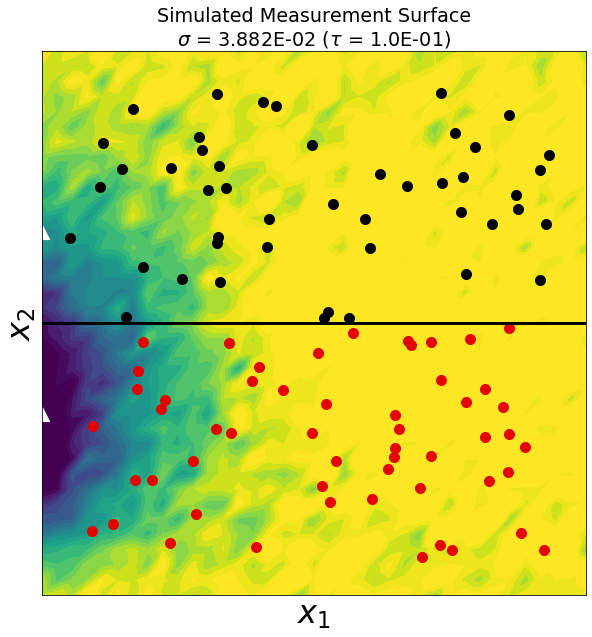
\includegraphics[width=0.475\linewidth]{figures/pde-highd/pde-highd_sensors_D2.png}
  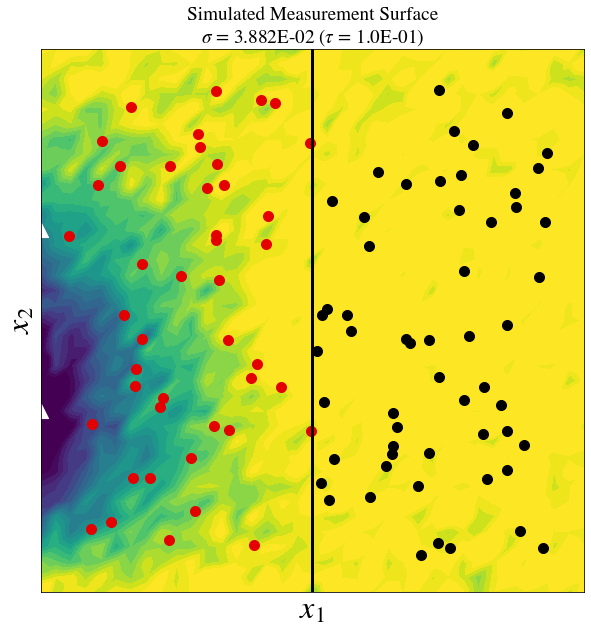
\includegraphics[width=0.475\linewidth]{figures/pde-highd/pde-highd_sensors-alt_D2.png}
  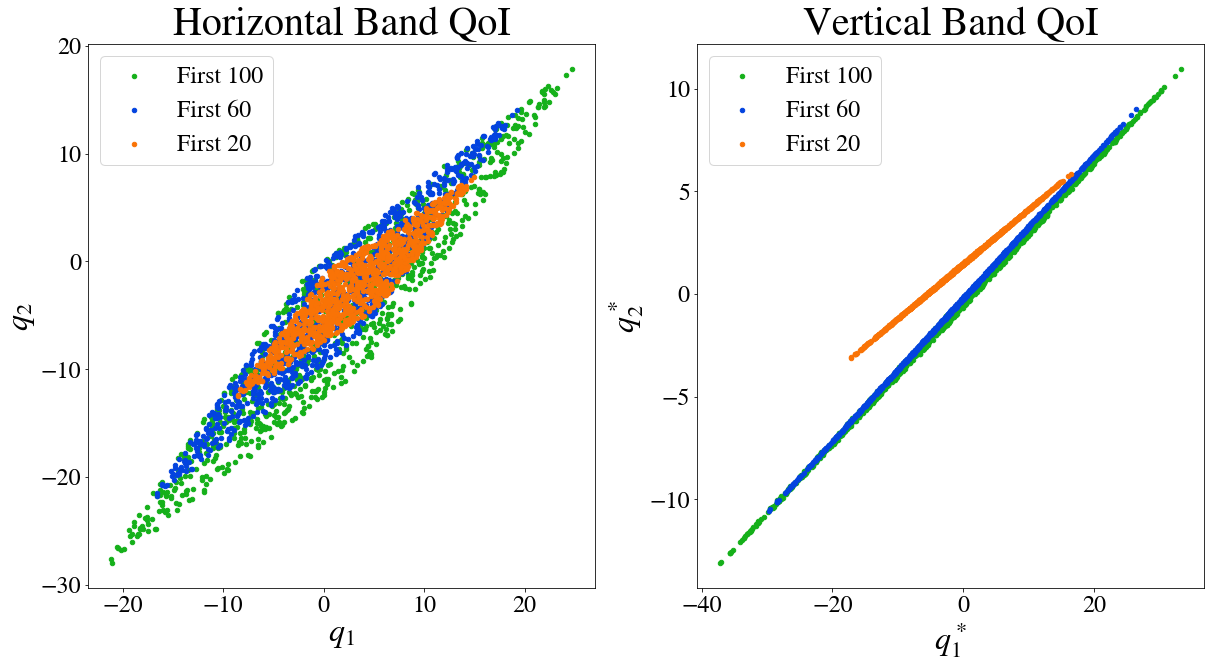
\includegraphics[width=0.95\linewidth]{figures/pde-highd/pde-highd_geom_D2.png}
\caption{
(Bottom): The vector-valued QoI map is constructed for all $N=10,000$ parameter evaluations and the two resulting vectors are plotted against one another for both methods of partitioning $\Omega$.
}
\label{fig:pde-highd-2d-geometry}
\end{figure}

The choice of which partitioning method to use is akin to the following question:
\begin{center}
\emph{With two QoI maps under consideration, which should we use?}
\end{center}

We use heuristics and an understanding of skewness to help address this question.
We first sample the predicted data spaces using simulated spatial data associated with $1000$ parameter samples to build intuition about the underlying geometry induced by these maps.

[TK - motivate WHY you are about to do this. Predicted vs. Observed, What is happening?]

[TK - rewrite the whole subset of measurements process more clearly.]
We repeat this process for three subsets of the measurements (using the first samples in each half of $\Omega$ according to the random index assigned to them), and demonstrate the two resulting sets of relationship in the bottom half of Figure~\ref{fig:pde-highd-2d-geometry}.
This figure also shows the associated designs against the noisy response surface as a backdrop.

First, we note that the inclusion of more data points has the effect of dilating (and to some extent rotating) the induced data space for both QoI maps.
Recall that the observed distribution remains a standard Gaussian, regardless of the number of data points used to construct the map.
In two dimensions, this observed distribution becomes a multivariate normal distribution instead, which can be visually thought of as a circular ``target'' located in the middle of each of the scatter-plots in Fig.~\ref{fig:pde-highd-2d-geometry}.
As more measurements are incorporated, the size of that target relative to the rest of the space becomes increasingly small since the data manifolds dilate.
Another analogy is of trying to find a needle in successively larger piles of hay.
More work is required to find a good solution to the SIP, since there are more measurements with which the model must agree.

The second implication of the two ways in which the maps can be formed is more visually evident, as the two quantities of interest that arise from a vertical bisection of $\Omega$ are nearly perfectly correlated.
In other words, $\qoi^\text{2D}_\prime$ has much higher skewness than $\qoi^\text{2D}$.
The two maps are presenting almost the same information (the shapes are very slim parallelograms), and so we fundamentally can already expect there to be very little difference between MUD points arising from using this map when compared to using the scalar--valued map.

By contrast, the map induced by a horizontal split (bottom left of Fig. \ref{fig:pde-highd-2d-geometry}) provides new information in each component.
While there is some correlation (the manifolds are not rectangular), a far greater proportion of samples will fall within the practical support of the observed distribution, which qualifies them as possible solutions to the SIP.
More information is learned with the inclusion of each component using this design than would be with the vertical split.
Had we performed an analysis of average skewness, we could have discovered these geometric implications without visual inspection.
Using a quantitative measure such as skewness allows us to scale the assessment to higher-dimensional parameter space.

We focus attention on comparing higher-dimensional QoI maps constructed from aqggregating data separated into more horizontal bands to scalar QoI maps (as proxies for highly-skewed maps), and note that a more thorough discussion of constructing QoI maps that induce desirable geometric properties is of interest for future work.
In \ref{sec:mud-higher-dimensions}, the ``vector--valued'' map will refer to the one with data aggregated into separate horizontal bands.
We note that this design, while not guaranteeing optimality for precision or accuracy's sake, respects the flow of information in the system being studied.
Since the parameter represents the left Neumann boundary condition, information about its state flows from left to right in the horizontal direction.

\FloatBarrier
